% Copyright (c) 2008-2009 solvethis
% Copyright (c) 2010-2016,2018-2019,2021 Casper Ti. Vector
% Copyright (c) 2021 Kurapica
% Public domain.
%
% 使用前请先仔细阅读 pkuthss 和 biblatex-caspervector 的文档,
% 特别是其中的 FAQ 部分和用红色强调的部分。
% 两者可在终端/命令提示符中用
%   texdoc pkuthss
%   texdoc biblatex-caspervector
% 调出。

% 如果格式审查提示字号不严格符合标准,可以在 [] 中加入“ugly”选项。
\documentclass[UTF8]{pkuthss}
% 如果的确须要使脚注按页编号的话,可以去掉后面 footmisc 包的注释。
%\usepackage[perpage]{footmisc}

% 使用 biblatex 排版参考文献,并规定其格式(详见 biblatex-caspervector 的文档)。
% 这里按照西文文献在前,中文文献在后排序(“sorting = ecnyt”);
% 若须按照中文文献在前,西文文献在后排序,请设置“sorting = cenyt”;
% 若须按照引用顺序排序,请设置“sorting = none”。
% 若须在排序中实现更复杂的需求,请参考 biblatex-caspervector 的文档。
% biblatex-caspervector 也有一个“ugly”选项,使其更像国标格式;此外也可考虑
% 改用 style = gb7714-2015 并去掉之后两选项,详见 biblatex-gb7714-2015 的文档。
\usepackage[backend = biber, style = caspervector, utf8, sorting = none]{biblatex}
\usepackage{amsmath}
\usepackage{algorithm}
\usepackage{algorithmicx}
\usepackage[noend]{algpseudocode}
\usepackage{diagbox}
\usepackage{listings}

\hypersetup{hidelinks}

% 对于 linespread 值的计算过程有兴趣的同学可以参考 pkuthss.cls。
\renewcommand*{\bibfont}{\zihao{5}\linespread{1.27}\selectfont}
% 按学校要求设定参考文献列表的段间距。
\setlength{\bibitemsep}{3bp}

\newcommand{\tabincell}[2]{\begin{tabular}{@{}#1@{}}#2\end{tabular}}

% 如是双盲版论文,将 \blindfalse 改为 \blindtrue。后面可用
% \ifblind 根据是否双盲来条件地启用代码(参见本文件后面部分)。
\newif\ifblind\blindfalse
% 设定文档的基本信息。
\pkuthssinfo{
	cthesisname = {博士研究生综合考试报告}, ethesisname = {Ph.D. Qulifaction Thesis},
	thesiscover = {博士研究生综合考试报告},
	% 长标题可用 \newline 强制换行,不能用“\\”(双盲版会出错)。
	ctitle = {云计算与人工智能相关技术研究},
	etitle = {Research on Artifical Intelligence in the Environment of Cloud Computing},
	cauthor = {李炎}, eauthor = {Yan Li}, date = {二〇二一年五月},
	studentid = {2001111305}, school = {信息科学技术学院},
	cmajor = {计算机软件与理论}, emajor = {Computer Software and Theory},
	direction = {云计算与普适计算},
	cmentor = {梅宏}, ementor = {Prof.\ Hong Mei},
	ckeywords = {云计算,人工智能,机器学习,新硬件},
	ekeywords = {Cloud Computing , Aitifical Intelligence, Machine Learning, New Hardware},
	% 以下两项无双盲评审需求的用户可保持原状。
	blindid = {9876543210}, discipline = {某某学科}
}
% 载入参考文献数据库(注意不要省略“.bib”)。
\addbibresource{thesis.bib}

% 普通用户可删除此段,并相应地删除 chap/*.tex 中的
% “\pkuthssffaq % 中文测试文字。”一行。
\usepackage{color}
\def\pkuthssffaq{%
	\emph{\textcolor{red}{pkuthss 文档模版最常见问题:}}

	\texttt{\string\cite}、\texttt{\string\parencite} %
	和 \texttt{\string\supercite} 三个命令分别产生%
	未格式化的、带方括号的和上标且带方括号的引用标记:%
	\cite{test-en},\parencite{test-zh}、\supercite{test-en, test-zh}。

	若要避免章末空白页,请在调用 pkuthss 文档类时加入 \texttt{openany} 选项。

	如果编译时不出参考文献,
	请参考 \texttt{texdoc pkuthss}“问题及其解决”一章
	“上游宏包可能引起的问题”一节中关于 biber 的说明。

	因无法假定用户使用哪种方式排版表格,用户须自行保证表格字号符合学校规定。%
}

\begin{document}
	% 以下为正文之前的部分,默认不进行章节编号。
	\frontmatter
	% 此后到下一 \pagestyle 命令之前不排版页眉或页脚。
	\pagestyle{empty}
	% 自动生成封面。
	\ifblind\makeblind\else\maketitle\fi
	% 版权声明。封面要求单面打印,故须新开右页。
	\cleardoublepage
	%\include{chap/copy}

	% 此后到下一 \pagestyle 命令之前正常排版页眉和页脚。
	%\cleardoublepage
	\pagestyle{plain}
	% 重置页码计数器,用大写罗马数字排版此部分页码。
	\setcounter{page}{0}
	\pagenumbering{Roman}
	% 中西文摘要。
	% Copyright (c) 2014,2016 Casper Ti. Vector
% Public domain.

\begin{cabstract}
	%\pkuthssffaq % 中文测试文字。
	21世纪10年代以来,云计算和人工智能可谓计算机科学领域最为炙手可热的两个研究方向。以虚拟化、资源管理和服务化为代表的云计算核心技术在近十余年里取得了丰硕的研究成果。当前,云计算已成为工业化社会重要的信息基础设施,支撑并推动着大数据和人工智能产业的快速发展。与此同时,人工智能技术在近十年内也相继在计算机视觉、自然语言处理等多个领域取得了突破,“智能化”已然成为现代社会的重要标签之一。
	
	本文将以上述两大技术的蓬勃发展为背景,研究云计算与人工智能相互影响、相互支持、相辅相成的相关技术。本文将按照如下几章展开。
	
	第一章对相关的技术背景做出简单介绍。
	
	第二章开始探究二者的关系。本章从“服务于系统架构的AI技术”这一视角展开,研究人工智能对云计算的增强技术。
	
	第三章从另一角度,研究云计算环境中用以支持人工智能的系统软件相关技术。
	
	第四章讨论近些年来云环境下出现的新硬件,如GPU,AI专用芯片,Intel-SGX等,为人工智能技术带来的新的机遇与挑战。
	
	第五章总结了上述三个方向的重要文献和相关研究团队概况。
	
	第六章介绍了作者下一步的研究计划。

\end{cabstract}

%\begin{eabstract}
%	Test of the English abstract.
%\end{eabstract}

% vim:ts=4:sw=4

	% 自动生成目录。
	\tableofcontents

	% 以下为正文部分,默认要进行章节编号。
	\mainmatter
	% 各章节。
	% Copyright (c) 2014,2016,2018 Casper Ti. Vector
% Public domain.

\chapter{引言}
%\pkuthssffaq % 中文测试文字。

\section{云计算的基本概念}

云计算(Cloud Computing),根据美国国家标准技术研究所(NIST)的定义,指的是一种可以实现对可配置计算资源共享池(如网络、服务器、存储、应用和服务)进行随时随地、便捷、按需网络访问的模型。这些资源可以迅速地配分配和释放,并且这个过程只需要最低限度的资源管理工作以及与服务提供商最少的交互。美国亚马逊公司再2006年3月推出了 Amanzon Web Service(AWS)\parencite{aws},这一事件一般被认为代表着云计算时代的正式开启。经过十几年的发展,凭借着“方便易用、弹性伸缩、按需服务”的技术特征,云计算概念已被广泛接受,云计算产业取得了商业上的巨大成功,云计算平台已成为当今社会的关键信息基础设施,云计算技术为大数据、人工智能的领域的蓬勃发展提供了重要的支撑作用。

\subsection{云计算的传统服务模型}

NIST 将云计算分为了三种服务模型。

这三种服务模型分别是基础设施即服务(Infrastructure as a Service,IaaS)、平台即服务(Platform as a Service,PaaS)以及软件即服务(Software as a Service,SaaS)。IaaS为消费者提供用来运行应用的计算资源,包括服务器、存储、网络等。其中虚拟机是云厂商提供的最核心的IaaS产品。与IaaS只提供最基础的底层资源不同,PaaS强调为消费者提供云开发环境,除计算资源以外,PaaS为用户提供中间件开发,运行平台及工具,帮助用户更方便地开、管理、测试和运行应用。SaaS是厂商提供的基于云的软件,用户无需下载安装软件,通过浏览器即可访问服务。

图\ref{rep_products}给出了云计算三种服务模型的代表产品。亚马逊公司的AWS EC2\parencite{awsec2},谷歌公司的Google Compute Engine\parencite{googlecloud}以及阿里云公司的ECS\parencite{aliecs}都是典型的IaaS产品。其主要服务形态是云厂商向消费者售卖虚拟机或者裸金属服务器以及连带的网络、存储等附属产品。PaaS的代表性产品包括AWS Beanstalk、Google App Engine、Microsoft Azure App Servics等。此类产品为用户提供在云中快速部署和管理应用的能力,提供包括应用扩容,负载均衡,应用监控和安全管理等功能。相比于IaaS仅售卖以虚拟机为主的基础设施,PaaS降低了用户开发、管理、运维应用的成本,使得用户可以更加专注于构建应用本身。在云计算已经发展了十几年的当今时代,越来越多的SaaS产品涌现了出来。谷歌公司开发的Google Docs、Google Maps以及微软公司开发的Microsoft Office 365都是典型的SaaS产品。以Google Docs为例,与传统的文件处理办公软降相比,用户无需在本地花费大量存储空间来安装软件,只需要打开浏览器,输入URL,即可使用Google Docs服务处理文件,并且所有的文件都会被及时同步保存到云端。另一个代表性的SaaS产品是Google Maps。Google Maps与Google Docs类似,为个人用户提供在浏览器中直接使用的地图服务。与传统软件相比,SaaS在使用方式上具有方便灵活,跨平台的特性,同时用户存储在云端的数据经过云厂商的冗余备份也具有更高的可靠性。

\begin{figure}
    \centerline{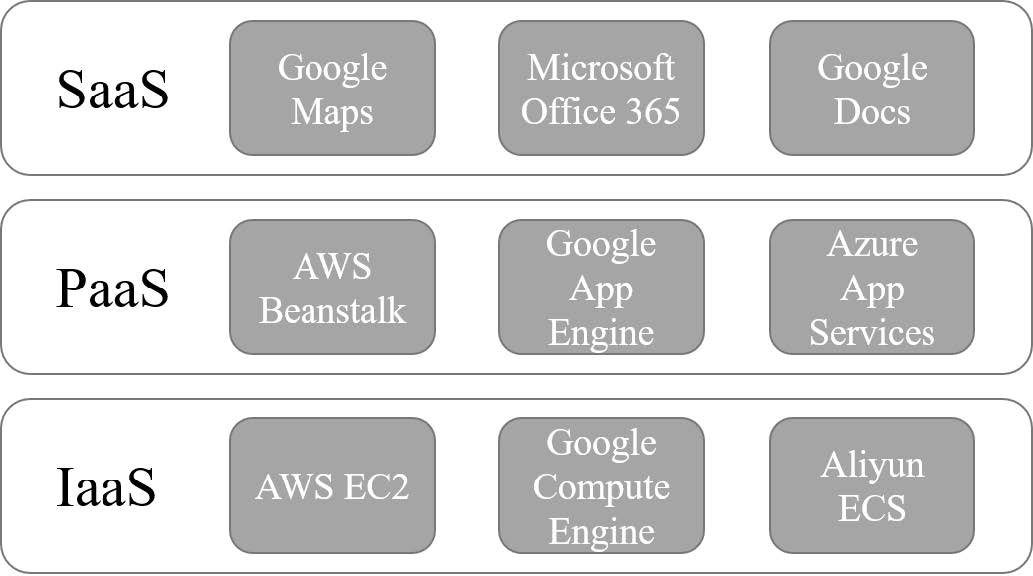
\includegraphics[width=\textwidth]{figures/rep_products.jpg}}
    \caption{云计算服务模型代表产品}
    \label{rep_products}
\end{figure}

\subsection{云计算的新兴服务模型}

云计算发展至今日,其服务模型已经不严格局限于NIST最初总结的这三种基本形态,世界各地各领域的研究者们已经提出了众多不同的X as a Service,包括Blockchain as a Service\parencite{samaniego2016blockchain},Sensing as a Service\parencite{perera2014sensing},Workspace as a Service\parencite{an2017workspace}等。与传统的三种服务形态相比,这些服务不单纯是硬件服务或者软件服务,其结合二者的特点,面向特定的领域方向进行更深度的定制,如区块链、物联网、分布式共识等。服务形态的日益丰富,服务内容的日益复杂体现了云计算更见领域化,精细化的发展趋势。而近几年来最热门的概念莫过于FaaS,即Fucntion as a Service\parencite{baldini2017serverless}。

FaaS是一种新兴的计算模式,亦被称为Serverless Computing。从字面理解,Serverless Computing即为“无服务器计算”之意。然后,其并非意味着真的没有服务器,而已说开发者不用过多考虑服务器的相关问题。在传统的IaaS服务中,开发者需要自己惊醒服务器管理与运维,负责服务的发布,在流量变化时对服务器集群进行扩容或缩容。而在FaaS中,开发者只需要关注业务逻辑,至于服务的发布、管理、弹性伸缩等,则交由云厂商来完成。

FaaS背后的机制一般是以容器技术为基础的。典型地,开发者上传自己的业务代码后,云厂商并不会直接收费。当对该服务的请求到来之时,云厂商将启动一系列容器来运行该服务,从而对用户的请求进行响应。通常而言,开发者指定的服务会与某些时间绑定(hook),在发生该事件时,立即触发开发者定义的服务。我们以AWS的serverless computing服务Lambda\parencite{klems2018aws}中的一个示例程序为例,讲述整个流程。图\ref{aws_resize}所示的是一个为照片调整大小的服务。该服务与AWS S3(AWS的对象存储服务)的上传事件绑定,当云厂商检测到有用户向S3上传图片时,会立即触发开发者定义的图片大小调整函数。整个流程中,开发者需要关注的只有第四步的函数开发工作,至于该函数的横向拓展,全部由云厂商来负责。

\begin{figure}
    \centerline{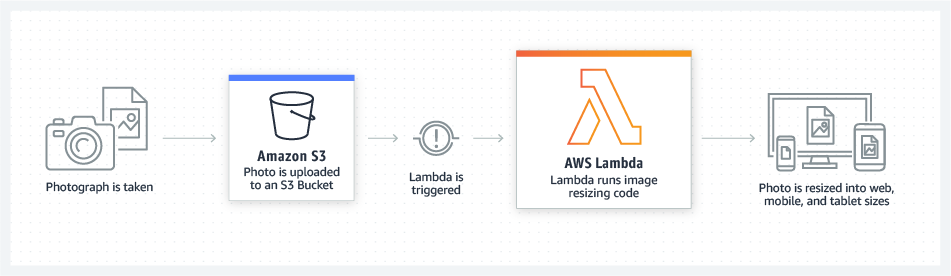
\includegraphics[width=\textwidth]{figures/aws-lambda-resize.png}}
    \caption{AWS Lambda中示例程序:照片大小调整}
    \label{aws_resize}
\end{figure}

主流的云厂商均提供了FaaS服务,例如AWS的Lambda,阿里云的函数计算等,近年来越来越受到开发者的青睐。一方面是因为它的高弹性,易于开发。另一方面则是因为其细粒度的收费模式。通常而言,FaaS的服务是按照请求次数进行收费。当函数闲置时,并不产生额外的费用。

\section{人工智能技术发展简介}\label{sec_ml_history}
人工智能是一个范围很广的概念,广义上的人工智能泛指通过计算机(机器)来实现人的头脑思维,使得机器像人一样区做决策。机器学习是实现人工智能的一种技术途径。一般可以认为人工智能的发展和机器学习技术的进步是同步的,因此,这两个概念大多数场景下会出现在同一个语境中。根据机器学习的发展史,即可勾勒出人工智能领域的发展轨迹,因此本节将简介机器学习技术的发展简史。

虽然机器学习这一名词以及其中某些零碎的方法可以追溯到1958\parencite{samuel1995some}年甚至更早,但真正作为一门独立的学科要从1980年算起,在这一年诞生了第一届机器学习的学术会议和期刊。到目前为止,机器学习的发展经历了3个阶段:1980年代是正式成形期,尚不具备影响力。1990-2010年代是蓬勃发展期,诞生了众多的理论和算法,真正走向了实用。2012年之后是深度学习时期,深度学习技术诞生并急速发展,较好的解决了现阶段AI的一些重点问题,并带来了产业界的快速发展。

\subsection{1980s:登上历史舞台}
十九世纪八十年代,机器学习作为一股独立的力量开始登上历史舞台。此后的十年内,出现了一些重要的方法和理论,典型的代表是:分类与回归树\parencite{breiman1983classification}、反向传播算法\parencite{rumelhart1986learning}和卷积神经网络\parencite{lecun1989backpropagation}。

\textbf{分类与回归树。}分类与回归树由L. Breiman等人在1984年提出,是决策树的一种经典实现,至今它还在很多领域里被使用。决策树是一种基于规则的方法,它由一系列嵌套的规则组成一棵树,完成判断和决策。和之前基于人工规则的方法不同,这里的规则是通过训练得到的,而不是人工总结出来的。

\textbf{反向传播算法。}人工神经网络是对动物神经系统的一种简单模拟,属于仿生方法。从数学的角度看,它是一个多层的复合函数。反向传播算法是神经网络训练时使用的算法,来自于微积分中复合函数求导的链式法则,至今深度学习中各种神经网络的训练使用的还是这种方法。反向传播算法的出现使得多层神经网络真正成为一种可以实现、具有实用价值的算法。在这一时期,神经网络的理论性研究也是热门的问题,神经网络数学上的表达能力的分析和证明大多出现在1980年代末和1990年代初。

从理论上来说,加大神经网络的规模可以解决更复杂的模式识别等问题。但是网络层数的增加会导致梯度消失问题,另外神经网络还面临着局部最优解的问题。训练样本的缺乏,计算能力的限制,都使得神经网络在接下来的20多年里没有太大的进展和出色的表现。

\textbf{卷积神经网络。}早在1989年,Y. LeCun在贝尔实验室就开始使用卷积神经网络识别手写数字\parencite{lecun1989backpropagation},这是当前深度学习中深度卷积神经网络的鼻祖;1998年,LeCun提出了用于字符识别的卷积神经网络LeNet5,并在手写数字识别中取得了较好的结果。卷积神经网络借鉴了动物视觉神经系统的原理,它能够逐层的对输入图像进行抽象和理解。

\subsection{1990-2012:走向成熟和应用}
在这一阶段的20余年里,机器学习的理论和方法得到了完善和充实,代表性的工作包括:支持向量机(SVM)\parencite{cortes1995support}、AdaBoost算法\parencite{freund1995boosting}、循环神经网络(RNN)和长短时记忆网路(LSTM)\parencite{hochreiter1997long}、流形学习\parencite{roweis2000nonlinear}以及随机森林\parencite{breiman2001random}。

\textbf{SVM。}SVM基于最大化分类间隔的原则,通过核函数巧妙的将线性不可分问题转化成线性可分问题,并且具有非常好的泛化性能。和神经网络相比,SVM有完善的数学理论作为支撑,训练时求解的问题是凸优化问题,因此不会出现局部极值问题。

\textbf{AdaBoost。}AdaBoost和随机森林同属集成学习算法,它们通过将多个弱学习器模型整合可以得到精度非常高的强学习器模型,且计算量非常小。AdaBoost算法在机器视觉领域的目标检测问题上取得了成功,典型的代表是人脸检测问题。2001年,使用级联AdaBoost分类器和Haar特征的算法在人脸检测问题上取得了巨大的进步,是有里程碑意义的成果。此后这一框架成为目标检测的主流方法,直到后来被深度学习取代。

\textbf{循环神经网络。}循环神经网络作为标准前馈型神经网络的发展,具有记忆功能,在语音识别、自然语言处理等序列问题的建模上取得了成功,是当前很多深度学习算法的基础。

\textbf{流形学习。}
流形学习作为一种非线性降维技术,直观来看,它假设向量在高维空间中的分布具有一定的几何形状。在2000年出现之后的一段时间内名噪一时,呈现出一片繁荣的景象,但在实际应用方面缺乏成功的建树。

\textbf{随机森林。}
随机森林由Breiman等人在2001年提出,是多棵决策树的集成,在训练时通过对样本进行随机抽样构造出新的数据集训练每一棵决策树。它实现简单,可解释性强,运算量小,在很多实际问题上取得了相当高的精度。时至今日,在很多数据挖掘和分析的比赛中,这类算法还经常成为冠军。

在这一时期机器学习算法真正走向了实际应用。典型的代表是车牌识别,印刷文字、(OCR),手写文字识别,人脸检测技术(数码相机中用于人脸对焦),搜索引擎中的自然语言处理技术和网页排序,广告点击率预估(CTR),推荐系统,垃圾邮件过滤等。

\subsection{2012之后:深度学习时代来临}
在与SVM的竞争中,神经网络长时间内处于下风,直到2012年\parencite{krizhevsky2017imagenet}局面才被改变。SVM、AdaBoost等所谓的浅层模型并不能很好的解决图像识别,语音识别等复杂的问题,在这些问题上存在严重的过拟合。为此产业界需要更强大的算法,历史又一次选择了神经网络。

由于算法的改进以及大量训练样本的支持,加上计算能力的进步,训练深层、复杂的神经网络成为可能,它们在图像、语音识别等有挑战性的问题上显示出明显的优势。

深度学习的再度兴起可以追溯到2006年,G. Hinton等人\parencite{hinton2006reducing}提出了一种训练深层神经网络的方法,用受限玻尔兹曼机训练多层神经网络的每一层,得到初始权重,然后继续训练整个神经网络。2012年Hinton小组发明的深度卷积神经网络AlexNet\parencite{krizhevsky2017imagenet}首先在图像分类问题上取代成功,随后被用于机器视觉的各种问题上,包括通用目标检测,人脸检测,行人检测,人脸识别,图像分割,图像边缘检测等。在这些问题上,卷积神经网络取得了当前最好的性能。在另一类称为时间序列分析的问题上,循环神经网络取得了成功。典型的代表是语音识别,自然语言处理,使用深度循环神经网络之后,语音识别的准确率显著提升,直至达到实际应用的要求。

与此同时,在策略、控制类问题上,深度强化学习技术取得了成功,典型的代表是AlphaGo\parencite{silver2016mastering}。在各种游戏、自动驾驶等问题上,深度强化学习显示出了接近人类甚至比人类更强大的能力。另外,以生成对抗网络(GAN)\parencite{goodfellow2014generative}为代表的深度生成框架在数据生成方面取得了惊人的效果,可以创造出逼真的图像,流畅的文章,动听的音乐,为解决数据生成这种“创作”类问题开辟了一条新思路。这一时期AI的产业化明显加速,人工智能已经成为当前计算机科学领域最炙手可热的方向。随着机器学习任务的规模越来越大,其对算力的要求也越来越高,大量机器学习任务开始向有着近乎无限资源的公有云迁移。

\section{云计算和人工智能交叉领域的常见研究问题}
云计算和人工智能是两个息息相关的热门领域。一方面,以深度学习为典型代表的人工智能技术在当今社会被应用的越来越广泛,研发、调试、发布新的模型的需求日益增长。与这种发展趋势对应,多数主流的云厂商都提供了机器学习模型训练-测试-部署的pipeline。学术界也不断探索“云上机器学习”这一话题,在各种不同的业务场景下,利用不同的云服务更便捷、更经济高效地在公有云上开展ML模型的训练和部署。同时得益于近年硬件技术的发展,多种新硬件(多体现为人工智能的加速芯片)在云环境中得到应用,进一步方便机器学习用户将整个开发流程迁移到云端。另一方面,机器学习技术也越来越多被用于解决云计算中常见的问题。例如使用机器学习算法解决置优化问题和利用强化学习解云环境中的资源调度问题。下文对这几个常见问题做简单概述,具体研究将在后续几章展开。

\subsection{基于公有云服务的机器学习平台}
\textbf{1. 产业界}

主流的云厂商都提供了面向机器学习的平台系统,例如AWS和Sagamaker\parencite{joshi2020amazon,liberty2020elastic,perrone2020amazon},Azure的Azure ML Studio\parencite{etaati2019azure},腾讯的Angel\parencite{jiang2018angel}等。这些基于云的平台提供了一站式调试、训练和部署ML模型的能力。一般而言此类平台被视为SaaS类的服务,因为其是基于云资源构建的上层软件栈,使得用户能够直接使用web的方式使用。例如Sagemaker就支持用户直接在浏览器中用jupyter notebook编写和调试模型代码。

\textbf{2. 学术界}

一般而言,产业界的平台系统面向的是一般性用户的普遍需求。因此,对于有特殊需求的用户,通常会有与产业界的解决方案并行的工作。例如,为了以尽可能低的成本在云上完成模型的训练,相关工作\parencite{harlap2017proteus,li2020spottune}尝试利用云上的动态资源(价格低但是稳定性/可用性低)进行模型的训练,并辅以一定的策略增强其可靠性。再比如,机器学习模型的在线服务会有低延迟、高吞吐率的要求。为了实现上述需求,相关工作\parencite{zhang2019mark}利用云上的多种资源(如IaaS,FaaS等),根据负载的动态变化,敏捷地在不同资源之间切换,充分利用不同类型资源的优点,规避掉其缺点,实现高效、经济的模型在线服务。一般而言,学术界的此类研究构建于云厂商服务的上层,是一种Cloud-of-Clouds的模式。

\subsection{利用新的计算模式在云上运行机器学习pipeline}
以FaaS为代表的新型云计算模式,以其高弹性、灵活的计费方式等特点吸引了众多研究者的注意。一般而言,用来训练机器学习模型的集群大小是固定的,很难动态地进行伸缩。同时,开发者还需要自行对该集群进行维护和管理,从而徒增一些不必要地时间和人力开销。因此,学术界开始探讨如何使得机器学习工作流享用到FaaS的诸多优点\parencite{wang2019distributed},从而使得其计算资源在模型训练时能按需伸缩,结束训练后自动将模型存储在持久化存储中,计算资源随即释放。

除了模型训练,也有部分研究者尝试利用FaaS,以serverless的模式部署模型。虽然这一想法非常自然,但是还有诸多问题需要解决。例如,现有的serverless服务,如AWS Lambda,其单个instance所能使用的内存有限,也无法使用GPU等加速芯片,同时其冷启动时间也较长(相比于服务对latency的要求)。如何优化FaaS的系统架构,使其更适合模型的部署,也是一个值得研究的问题。

\subsection{异构硬件对人工智能的影响}
根据\ref{sec_ml_history}中的描述,人工神经网络早在上世纪80年代就被提出。然而直到本世纪10年代左右,神经网络才再次进入学术界和产业界的视野,并得到了飞速发展。除了理论的进步,更重要的原因是算力的大幅进步。以GPU,FPGA为代表的并行化加速硬件,极大地加快了深度学习模型的训练速度,使得学术界对于新模型架构的探索周期大幅缩短。在这种背景下,除了深度学习算法理论的迭代加快,也催生了一批针对机器学习系统的研究工作。这些工作关注如何使异构的硬件更好地支持机器学习模型的训练。

除了训练速度,安全也是人工智能领域的一个重要问题。当今时代数据已经成为重要的资产,开发者在将机器学习任务部署到云端的同时,也会对数据的安全性有所担忧。虽然诸如同态加密之类的软件层面的解决方案可以提升ML任务的安全性,但是由于性能的制约始终未能得到大规模应用。以Intel SGX\parencite{costan2016intel}为代表的安全计算环境技术,给人工智能安全带来了新的解决方案。

\subsection{利用机器学习算法解决配置优化问题}
公有云厂商所提供的计算资源类型和计费模式越来越复杂。据不完全统计,截至目前,AWS EC2提供了超过400种配置的虚拟机,阿里云提供了超过500种虚拟机。除了虚拟机配置不同之外,其收费模型也存在多种。例如,除了传统的包年包月、按量付费等,还有抢占式实例(在AWS中成为Spot Instance)\parencite{awsspot}等计费方式。在此场景中,用户所面临的一个重要问题在于如何为自己的应用程序/负载选择合适配置和收费方式的资源。

部分研究者利用机器学习算法来解决此类问题。有的将其看作一个推荐问题\parencite{klimovic2018selecta},用协同过滤等推荐系统中常用的算法为不同的应用程序匹配合适的配置。有的将其建模为回归问题\parencite{yadwadkar2017selecting,venkataraman2016ernest,moradi2019performance,zheng2019online},将应用程序的信息、资源的配置信息等作为输入,预测在某种配置下某个应用程序的性能或者花费,从而得到最佳的配置。还有的将其视作在线优化问题\parencite{alipourfard2017cherrypick,casimiro2019lynceus},利用贝叶斯优化等方法,通过有限次的尝试逐渐逼近最优解。

\subsection{利用机器学习算法解决资源调度问题}
资源调度是操作系统、分布式系统和云计算领域中的经典问题,其本质在于为系统中的每个任务分配合适的资源,从而使得系统达到某种状态,如资源利用率最高、闲置资源最少或者吞吐率最高等。近年来深度学习的流行,尤其是强化学习的兴起,使得部分研究者开始思考利用机器学习算法解决资源调度问题\parencite{delimitrou2014quasar,mao2019learning,chung2018stratus}。一般而言,此类算法旨在从过去的任务执行记录中“学习”相关的规律,以指导为未来系统的调度动作。
% vim:ts=4:sw=4

	% Copyright (c) 2014,2016 Casper Ti. Vector
% Public domain.

\chapter{面向人工智能的云计算系统软件研究}
% \pkuthssffaq % 中文测试文字。
以深度学习为代表性技术的人工智能领域在21世纪10年代再度兴起,社会各界对于人工智能的需求也愈发旺盛。遍布超市和餐馆中的扫脸支付技术、智能手机上的语音智能助手、工厂中检测废件的自动检测装置等,都离不开人工智能技术的加持。具体的,上述场景都需要适当的机器学习模型在线部署以提供服务。

机器学习的工作流一般遵循如下几个步骤:1)模型开发与调试。在此阶段中,开发者根据具体的场景,编写并调试模型代码。2)模型参数调整。在这个步骤中,开发者使用训练集不断调整模型的超参数,使其在测试集上的表现符合某种标准(如准确率高于某个阈值)。3)模型部署,开发者将开发完成的模型部署到对应的场景中对外提供服务。

为了方便开发者专注到模型的开发流程中,各大主流云厂商均实现了支持机器学习模型开发-调试-部署整个流程的软件栈。同时,云厂商提供的一般性的平台可能无法满足用户特定的需求。因此针对具体场景,学术界也提出了一系列基于云服务的机器学习软件,以达到降低开发成本、提高模型在线服务的质量等目标。本章对上述内容涉及到的相关工作展开具体研究。

\section{一站式的云上机器学习系统}

\subsection{AWS Sagemaker}
AWS作为公有云领域的龙头老大,在云计算的前沿技术领域一直处于领先的地位。其某些代表性技术甚至成为了多数公有云厂商所共识的标杆和规范。在机器学习系统这一分领域,其代表性系统为AWS Sagemaker。

Sagemaker是一个实现和产品化机器学习模型的框架\parencite{joshi2020amazon},用户可以将其模型训练需要的数据存储到AWS的对象存储服务S3中。然后,用户可以通过web的方式访问部署在云端的Jupyter Notebook服务,在线访问数据、编写并调试代码。当模型训练完毕后,可以使用Sagamaker内置的推理服务对模型进行发布。用户在发布时还可以根据平台的不同(云端或边缘节点)将模型打包编译成不同的版本。此外,Sagamaker还内置了一些常用的算法和数据集,方便开发者直接调用。

在训练算法和系统机制方面,Sagemaker旨在解决工业规模的模型训练场景中的如下几个常见问题:

\begin{itemize}
    \item \textbf{支持增量式的训练和模型更新。}在真实的工业场景中,几乎不存在完全静态的数据集。用来训练模型的数据集大多都是不断增长的。例如电商网站的用户行为数据,每天都在以相当的速度增长。在这样的动态数据上训练模型,势必要进行如下权衡:在全量数据上进行训练,可以获得质量更高的模型,然而时间和经济上的开销却会非常高;在最新更新的数据上(例如最近几天的数据)进行训练,可以快速的得到新的模型,却有可能在一定程度上牺牲模型的准确性。
    \item \textbf{容易估算训练模型产生的花销。}对于体量非常大的数据集,用户需要较为准确地估计训练模型将会产生的时间和经济花销。当今的云计算一般遵循按量付费的收费模式,因此云上的机器学习用户会格外关注花销的问题。
    \item \textbf{支持暂停和恢复模型训练,有一定的弹性。}生产环境中,大模型的训练通常包含跨越数十甚至上百台机器的并发任务。在一些场景中,由于超参数调整的需要或者计算资源的限制,开发者需要对这些任务进行中断和恢复。这就要求云上的ML系统能够支持大型训练任务中断和恢复时中间结果的保存和复原。
    \item \textbf{能够处理非持久性数据。}在很多场景中,数据并不一定是持久化的,也会有很多“瞬时”的数据,例如直播时的视频流等。这些数据一般不会被持久化保存,因此如何支持对这些数据的挖掘和学习也是一个重要的问题。
    \item \textbf{支持自动调参。}自动调参是一项非常耗时耗力的工作,特别是在生产环境的大数据集下。因此,如何能够支持高效的自动调参,方便用户选取合适的模型,对于云上的ML系统而言也是非常重要的。
\end{itemize}


\subsection{阿里云Max Compute}

\section{基于公有云服务的模型训练系统}

\subsection{基于云厂商动态资源的模型训练系统}
% harlap的第一篇工作

\subsection{基于云厂商动态资源的自动调参系统}
% SpotTune

\section{基于多种服务模式的模型部署系统}

\subsection{基于多种资源混用的模型部署系统}
% MArk

\subsection{基于FaaS的模型部署系统}
%一系列FaaS for ML serving的工作,INFaaS etc
% vim:ts=4:sw=4

	% Copyright (c) 2014,2016,2018 Casper Ti. Vector
% Public domain.

\chapter{云环境中的异构硬件为人工智能带来的机遇与挑战}
% \pkuthssffaq % 中文测试文字。
随着硬件技术的不断发展,云环境中支持机器学习任务的硬件也从单一的CPU变成了包含CPU、GPU、FPGA、TPU以及SGX等安全硬件的异构资源。利用这些异构资源,可以给机器学习任务带来一定增益。例如GPU,TPU和FPGA等硬件的SIMD计算模式天然适合ML这种迭代式、大批量的负载,从而可以大大加速ML训练。而诸如SGX等硬件由让机器学习安全有了从硬件层面得到解决的可能性。

而异构硬件为ML任务带来机遇的同时,也带来了一定的挑战。例如,在公有云共享资源池的背景下,如GPU和FPGA等新兴加速硬件没有成熟和系统的虚拟化方案,用户的使用这些硬件的模式仍然以独占为主。即便是共享,也没有成熟的隔离机制保证性能以及用户之间不会相互干扰。再比如,SGX加持的安全计算环境中,可信内存的大小十分有限,如何在有限的资源下支持可信的模型部署甚至模型训练,是亟待解决的问题。

本章将以加速型硬件GPU和安全型硬件SGX为主,介绍云环境中异构硬件为机器学习任务带来的机遇与挑战。

\section{云环境中机器学习作业对GPU的利用}

本节将先对GPU的现状做简要介绍,包括现代GPU的架构以及常见的GPU API和编程模型。然而,本章将从两个角度展开当前学术界针对ML任务对GPU的利用的研究:1)One Job on Multi GPUs。即一个ML任务需要多个GPU设备。这种情况一般出现在大型模型的分布式训练中。在一个大规模GPU集群中,不同的训练任务对GPU数量的需要可能不一样,如何对这些任务进行调度,使系统的资源利用率最高,同时保证训练任务的性能,是学术界研究的重点问题;2)Multi Jobs on one GPU。即在同一个GPU设备运行多个ML任务。这种情况在资源短缺或多租户的场景下较为常见。

\subsection{GPU简介}

\subsubsection{GPU架构}
GPU,即Graphics Processing Unit,采用了与传统的多核处理器完全不同的架构。GPU的设计围绕和让吞吐率最大化这一原则,提供了上千个简单的计算核心和高带宽内存。这样的实际使得GPU能够使一个应用程序拥有很高的并行度,从而使程序的吞吐率最大化。理想情况下,对于一个GPU应用程序,其包含的若干线程应该分别对应其数据空间的不同位置,而彼此之间由没有因果关联,从而可以并发地执行。与之相反,传统的处理器是为了能更快地执行线性的代码段而优化的。因此其单个核心的复杂度非常高,且单个处理器中的核心数量相对较少。且传统的处理器一般会使用复杂的控制逻辑和较大的本地缓存以处理传统程序中常见的条件分支、上下文切换以及较差的数据本地行。

\begin{figure}[h]
    \centerline{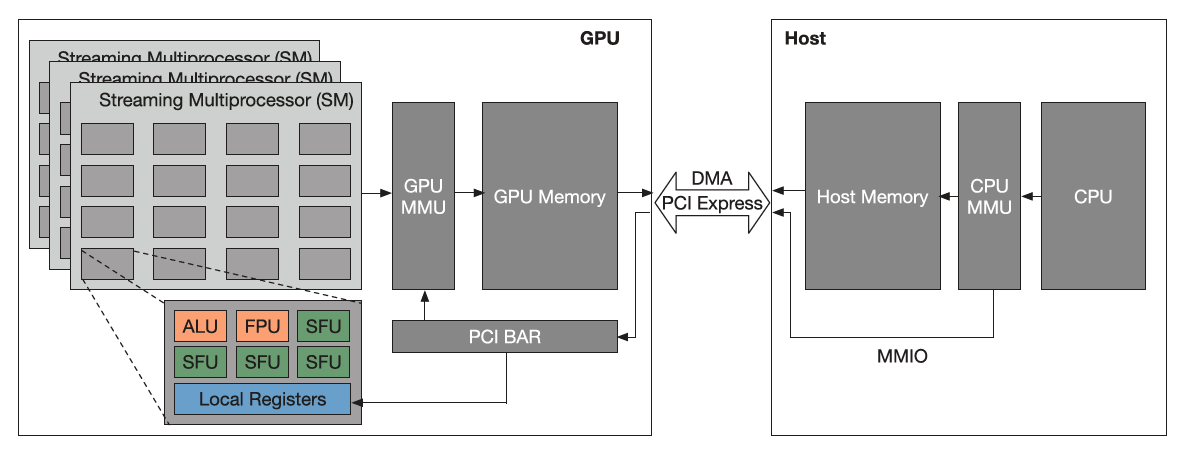
\includegraphics[width=\textwidth]{figures/gpu-arch.png}}
    \caption{GPU系统架构。}
    \label{gpu_arch}
\end{figure}

图~\ref{gpu_arch}展示了一个典型的GPU系统的架构。图中的GPU部分是根据Fermi架构的Nvidia GPU,但是现代的GPU(例如新一代的Nvida GPU和AMD GPU)也遵循类似的设计。一个GPU拥有多个流式处理器(streaming multiprocessor,SM),每一个SM拥有32个计算核心。每个SM也拥有L1数据缓存和低延迟共享内存。每个计算核心拥有本地的寄存器、一个整型计算单元(Integer Arithmetic Logic Unit,ALU)、一个浮点计算单元(Floating Point Unit,FPU)以及若干特殊函数单元(Special Function Units,SFU,用来计算特定的函数值,例如正弦函数sine和余弦函数cosine)。GPU的内存管理单元(MMU)为GPU程序提供虚拟地址空间。MMU会根据应用程序的页表,会将一个GPU地址解析为物理地址。

Host通过PCI高速通道(PCIe)与GPU连接。Host上的CPU通过内存输入/输出映射(MMIO)与GPU进行交互。GPU寄存器以及设备内存可以被CPU通过MMIO接口直接获取。此外,量比较大的数据交换可以通过DMA(Direct Memory Access)实现。DMA可以将数据在设备内存和主机内存之间快速传输。

\subsubsection{GPU API和编程模型}
常用的GPU API和编程模型包括OpenGL,Direct3D,CUDA和OpenCL等,在游戏开发、图像处理、高性能计算等场景下非常常用。

OpenGL是一个利用GPU硬件加速图形处理的库,通常应用于电子游戏、图像处理以及科学计算中的数据可视化。OpenGL实现了一个硬件无关的API,兼容适配不同的底层硬件。

Direct3D是由Microsoft Windows提供的图形库,通常在一些性能敏感的场景中(例如电子游戏)负责图形渲染工作。Direct3D同样实现了硬件无关的API,并且向用户暴露了能够使用GPU高级特性的API,例如Z-buffering,W-buffering等。

CUDA是由Nvidia提供了专为Nvidia GPU适配的并行加速库。CUDA允许开发者在GPU上利用高并行的特点开发特定的程序,这种情形下的GPU被称为GPGPU(General Purpose GPU)。CUDA API是与编程语言高度绑定的,例如C和C++。当前流行的机器学习框架,例如Tensorflow和Pytorch,在存在GPU设备的环境中,都支持利用CUDA对其模型训练进行加速。

OpenCL也是一个并行加速库,其基础功能和CUDA类似,最大的区别在于OpenCL可以被应用于非Nvidia的GPU。

\subsection{One Job on Multi GPUs: 机器学习集群中的GPU调度算法}
%SC 17 Topology-aware
%NSDI 19 Tiresias
%OSDI 20 HiveD
随着深度学习的兴起和快速发展,在计算机视觉、自然语言处理等领域使用的模型参数越来越多,规模越来越大。而对于大规模的深度学习模型,分布式训练+GPU硬件加持几乎成为了标配。分布式训练的场景中,GPU之间的数据传输时有发生。然而在一个多GPU的集群环境中,位于整个系统拓扑结构不同位置的GPU之间的数据传输速度是有很大差异的。

\begin{figure}[h]
    \centerline{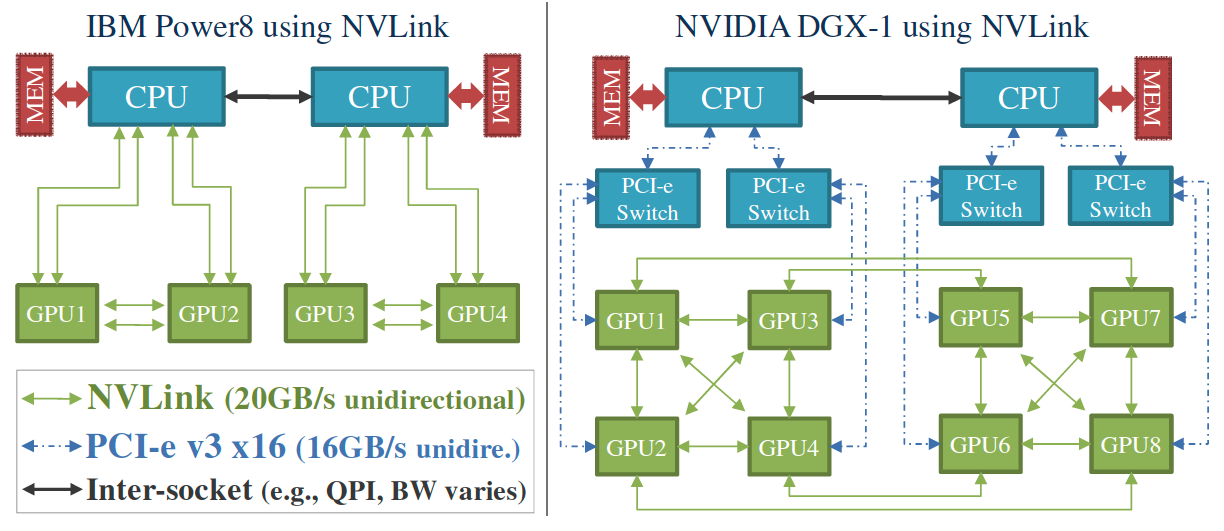
\includegraphics[width=\textwidth]{figures/gpu-topology.png}}
    \caption{GPU拓扑结构示例。}
    \label{gpu_topology}
\end{figure}

图~\ref{gpu_topology}展示了两个GPU服务器中GPU的和其它硬件之间的拓扑结构图。左图为IBM的Power8服务器,有两个CPU和四个GPU。右图嵬NVIDIA和DGX-1服务器,有两个CPU、四个PCI-e桥接器和8个GPU。绿色的线、蓝色的线和黑色的线分别代表NVLink、PCI-e和Intel的QPI三种连接方式,数据传输速度由快到慢。位于同一个CPU socket下的两个GPU(例如左图中GPU1和GPU2)之间的数据传输可以通过NVLink进行,是最快的。位于不同CPU上的GPU,只能通过PCI-e通道和QPI通道进行通信(例如左图中的GPU1和GPU3、右图中的GPU1和CPU)。而如果位于两台不同服务器上的GPU之间需要通信,则除了需要经过上述数据通路之外,还要经过网络传输,即时是万兆网(10Gbps),也要比上述传输方式慢约一个数量级。

\begin{figure}[h]
    \centerline{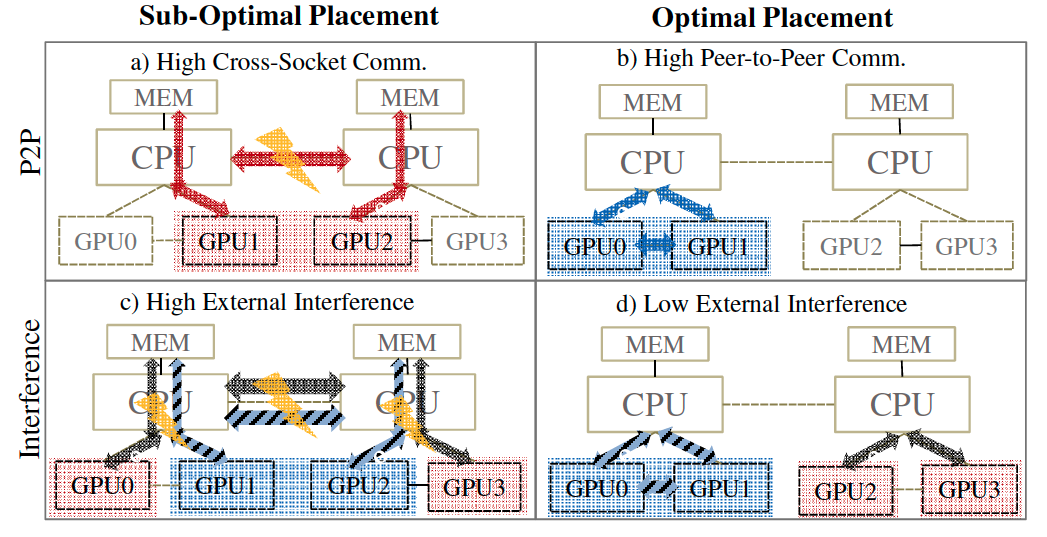
\includegraphics[width=\textwidth]{figures/gpu-top-sub-opt.png}}
    \caption{GPU调度示例。}
    \label{gpu_top_sub_opt}
\end{figure}

因此,在GPU集群中调度分布式ML训练任务时,需要充分考虑GPU之间的拓扑结构,否则可能会造成严重的性能损失。图~\ref{gpu_top_sub_opt}展示了GPU调度的两个例子和与其对应的四种调度方案。上面的两张图对应了P2P(即两个GPU之间需要互相通信)的场景中的两种调度方案,显然右边的方案是更优的方案,因为分配到的两个GPU位于同一个CPU socket上,于左边相比其数据通路具有更高的传输速率。下面的两张图对应了不当分配可能造成的性能干扰。显然,右边的分配方式也是更优的方式,因为左边的分配方式造成了两个Job在数据传输时共用同一条数据通路从而造成竞争,使性能降低。

M. Amaral等人\parencite{amaral2017topology}在2017年提出了一种云环境下基于GPU拓扑结构的调度方法。其将ML任务和集群都抽象成图的形式。在ML的任务图中,图的节点为GPU,节点之间的边代表两个GPU之间存在数据交流。任务图中的边没有权重。在集群的图中,图的节点为CPU,GPU,PCI-e桥接器,CPU socket或者网络交换机。不同节点之间的连线代表这两个节点之间可以相互通信,连线的权重代表通信速度,数值与越小通信速度越快。图~\ref{gpu_graph}表示了图~\ref{gpu_topology}所对应的拓扑结构图。

\begin{figure}[h]
    \centerline{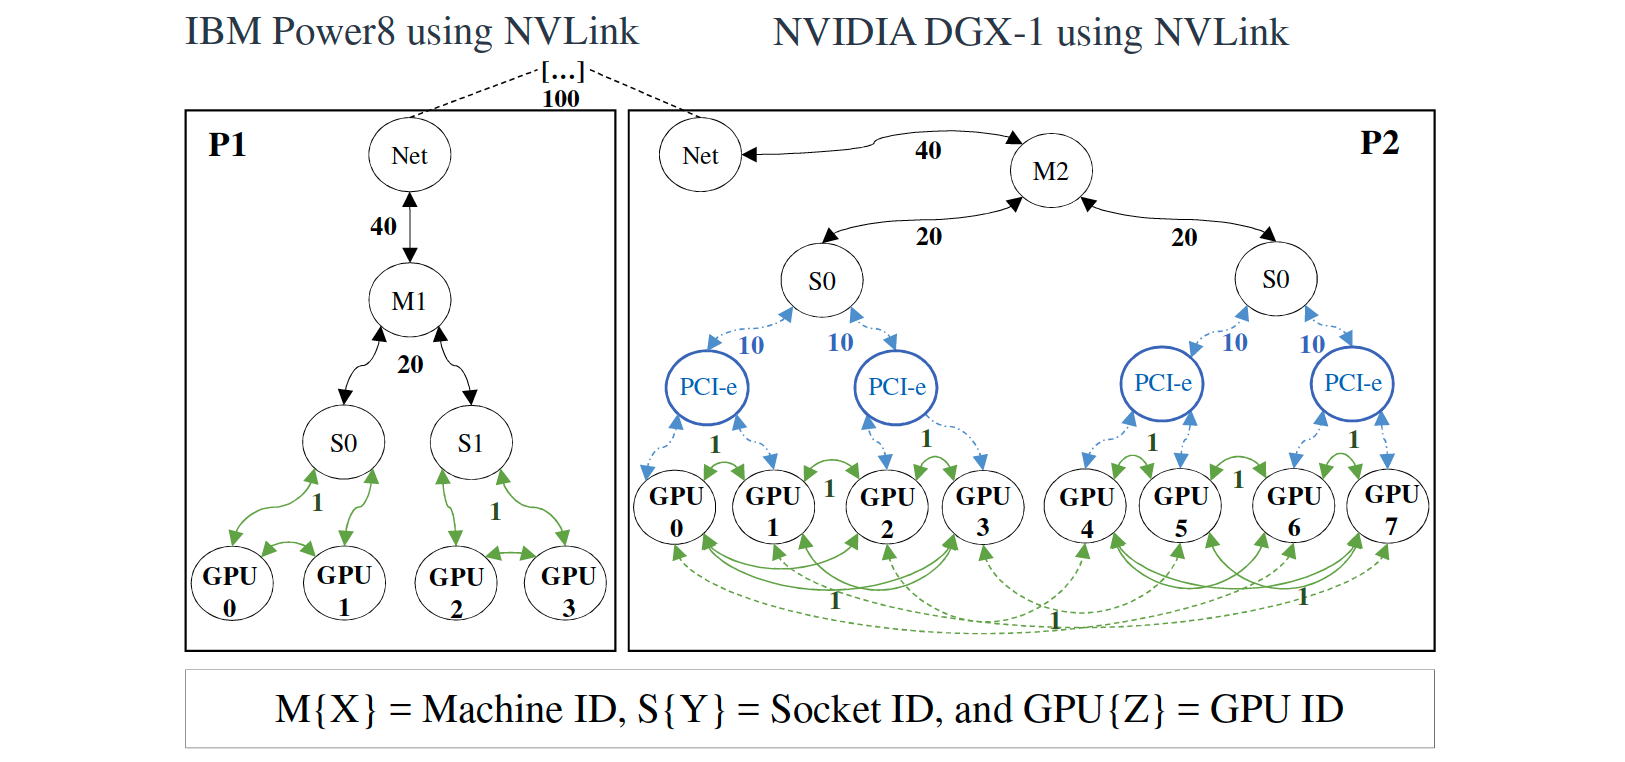
\includegraphics[width=\textwidth]{figures/gpu-graph.png}}
    \caption{GPU拓扑结构图。}
    \label{gpu_graph}
\end{figure}

M. Amaral等人通过对两个图进行匹配并最小化公式~\ref{eq_top_min}中的目标来实现GPU的调度,其中$\alpha^{cc}+\alpha^b+\alpha^d=1$,$t$、$I$和$\omega$分别代表GPU之间的通信代价、来自外部的资源干扰和资源碎片化程度,分子代表实际的值,分母代表最坏情况下的值。该公式旨在综合考虑减小GPU之间的通信代价、降低不同任务之间的干扰以及使整个系统的碎片化尽可能降低,使整个集群处于一个相对最佳的状态。

\begin{equation}\label{eq_top_min}
    MIN\ \alpha^{cc}\frac{t^{cc}}{t_w}+\alpha^b\frac{I^b}{I_w}+\alpha^d\frac{\omega^d}{\omega^w}
\end{equation}

\subsection{Multi Jobs on one GPU: 机器学习集群中的GPU共享机制}
%OSDI 18 Gandiva
%Eurosys 18 Optimus
%ASPLOS 20 SwapAdviosr
%MLSys 20 Salus
\section{云环境中机器学习作业对SGX的利用}

\subsection{SGX技术发展历程简介}

\subsection{在机器学习任务中应用SGX技术}

\section{小结}
% vim:ts=4:sw=4

	\chapter{人工智能对云计算的增强技术研究}
云计算中存在如下两个基本问题。第一,站在用户的视角,如何在浩如烟海的公有云资源池中选择最适合其应用程序的资源,即云配置优化问题。公有云厂商所提供的计算资源类型和计费模式越来越复杂。据不完全统计,截至目前,AWS EC2提供了超过400种配置的虚拟机,阿里云提供了超过500种虚拟机。除了虚拟机配置不同之外,其收费模型也存在多种。例如,除了传统的包年包月、按量付费等,还有抢占式实例(在AWS中成为Spot Instance)等计费方式。在此场景中,用户所面临的一个重要问题在于如何为自己的应用程序/负载选择合适配置和收费方式的资源。第二站在公有云运营商的角度,如何调度资源使其满足所有用户的需求,且达到一定的调度目标例如集群资源利用率最高、吞吐率最高等等。

近年来越来越多的学者尝试利用机器学习算法来解决上述两类问题。不同于前两章所述的公有云服务对机器学习负载的支持(Cloud for AI),本章将从“机器学习对云计算的增强技术”(AI for Cloud)着手,研究相关技术。
\section{基于机器学习算法的云资源配置优化技术}
自2010年AWS(Amazon Web Service)将云计算在产业界落地以来,各种云计算模型和应用层出不穷。云计算的高度弹性和海量的资源大大解放了开发者,使他们可以不用费时费力去关注数据中心的运维、物理节点的伸缩。受益于云计算的便捷性,公司、科研机构、事业单位都在将自己的负载向公有云上迁移。尽管云厂商提供了诸如IaaS、PaaS、SaaS、FaaS等各种云服务,但受限于绝大多数传统应用的架构和重构代价,大部分应用上云需求对准的都是基础的IaaS服务,即将部署在本地私有数据中心的应用迁移在云厂商提供的虚拟机上,以降低运维成本,并使原有的应用具备一定的弹性。

\begin{figure}[h]
    \centerline{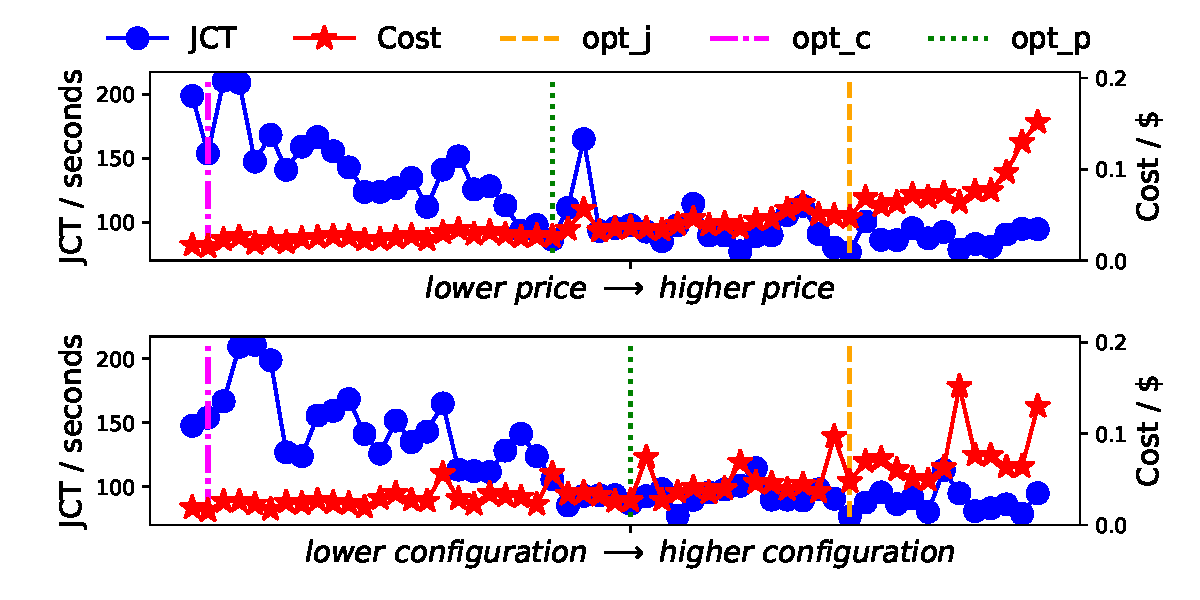
\includegraphics[width=\textwidth]{figures/mis_conf_effect.pdf}}
    \caption{同一任务在不同云配置下的性能和花费。}
    \label{mis_conf_effect}
\end{figure}

然而,即便云厂商帮助用户完成了集群维护、可靠性保障,但用户仍然需要在庞大的配置空间中选择最适合自己的应用和自己的需求的配置。而且,用户的需求各异,有的需要选择使得其应用完成时间尽可能短的配置,有的需要选择最终总花费尽可能少的配置,还有的可能综合考虑这两点,选择性价比最高的配置。如果仅凭一些启发式的规则,例如,选择配置最高的或者单价最低的,往往难以选择到最优的配置。图~\ref{mis_conf_effect}展示了Spark-Terasort这一任务在55种云资源配置上(跨越AWS、阿里云、腾讯云、华为云四大云厂商)的任务完成时间和总花费曲线。该图中,横轴代表不同的配置,其中上面的子图中,配置的单价由左到右单调递增,下面的子图中,配置的规则由左到右单调递增。opt\_j, opt\_c, opt\_p分别代表最优完成时间、最优花费和最优性价比,JCT为Job Completion Time的缩写,代表任务完成时间。很显然,最优的配置与直觉相违背。因此,此类用户需要一个自动选择最优配置的算法/工具,来帮助他们为自己的应用程序/负载选择最符合他需求(完成时间最短,总体花费最低或者性价比最高)的配置。

尝试解决此类问题的相关工作,其大体可以分为两类:1)数据驱动的线下建模方法;2)基于搜索的线上优化方法。本节按照这种分类方法介绍相关工作。

\subsection{数据驱动的线下建模方法}\label{sec_profling}

该类方法旨在通过在线下收集一系列形如 <meta data, performance> 的键值对,然后利用机器学习算法对上述键值对建立回归模型,以预测性能。其中meta data中可能既包括配置信息,如当前运行环境的硬件配置(CPU核数,CPU代数,memory大小等等),又包括可以刻画该workload的一些信息,如workload运行时某一时刻的CPU利用率等等。对于用户而言,使用该类算法的总体流程如图\ref{offline_profiling}所示。

\begin{figure}[h]
    \centerline{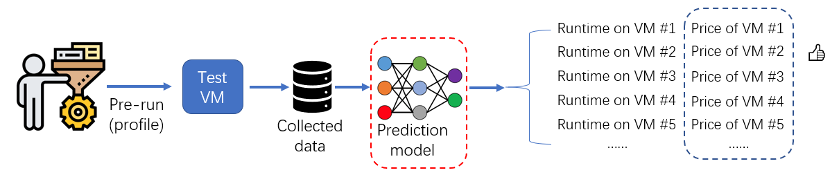
\includegraphics[width=\textwidth]{figures/offline_profiling.png}}
    \caption{数据驱动的线下建模方法流程图。}
    \label{offline_profiling}
\end{figure}

在模型训练阶段,需要对不同的workload在不同的VM上进行profile,形成形如<configuration, performance> 的键值对。然后对由该键值对构成的数据集进行模型训练。在预测阶段,用户需要在一个或者多个test VM上预运行自己的workload,并采集一些模型需要的数据,将其输入模型,并得到预测结果。该结果可能是该workload在配置集上所有VM配置上运行的性能数值或者最有的配置。总的来讲,该种类别中,不同的工作的主要区别在于上图中Prediction Model的结构。

\begin{figure}[h]
    \centerline{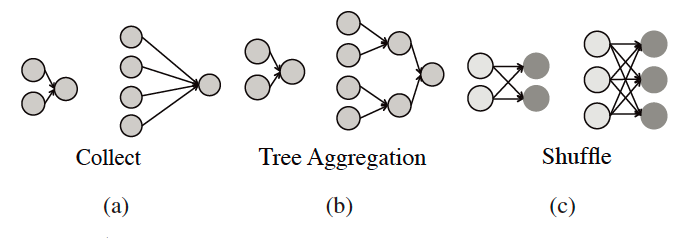
\includegraphics[width=\textwidth]{figures/ernest-data-flow.png}}
    \caption{Ernest中的三种数据流模式。}
    \label{ernest_data_flow}
\end{figure}

S. Venkataraman等人在2016年提出了Ernest\parencite{venkataraman2016ernest},可以称为云上性能建模的开山之作。Ernest主要关注Hadoop,Spark等基于map-reduce计算范式的应用程序。Ernest将基于map-reduce计算范式的程序中的数据流模式总结为如图~\ref{ernest_data_flow}所示的Collect、Tree Aggregation和Shuffle三种模式。其认为三种数据流模式的计算复杂度分别为$O(\frac{1}{machines})$,$O(machines)$和$O(log(machines))$, 因此使用公式~\ref{eq_ernest_model}对应用程序的性能进行拟合。虽然此模型非常简单,但是Ernest通过基于Spark-MLlib的实验证明了其模型可以达到较低的预测错误,且profile的代价较小。

\begin{equation}\label{eq_ernest_model}
    \begin{aligned}
    time =& \theta_0 + \theta_1 \times (scale \times \frac{1}{machines}) + \\
        &\theta_2 \times log(machines) + \\
        &\theta_3 \times machines
    \end{aligned}
\end{equation}

Ernest虽然可以达到较好的效果,但是其仅针对Hadoop和Spark等MR范式的应用,无法在一般性的场景中得到应用。且Ernest并未将资源配置作为输入参数,对于每种资源都需要使用模型建立一个单独的模型进行预测,在复杂的公有云中适用性较低。N. Yadwadkar等人在2017年提出了PARIS\parencite{yadwadkar2017selecting}。如图基于随机森林模型和两次预先运行收集到的数据对常用的数据处理任务进行性能建模。不同于Ernest,PARIS的输入参数除了资源信息,还包括预运行中收集到的关于当前应用程序的系统指标(最后一分钟、五分钟和十五分钟的系统指标,例如CPU利用率,内存利用率,中断次数等)。同时PARIS还不仅支持性能建模,还支持对花费进行建模。用户可以根据自己的需求,使用PARIS选择性能最优或者花费最低的云资源。

\begin{figure}[h]
    \centerline{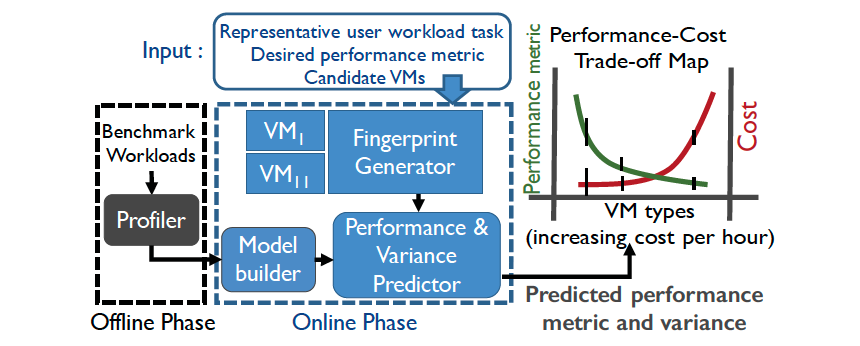
\includegraphics[width=\textwidth]{figures/paris-arch.png}}
    \caption{PARIS系统架构。}
    \label{paris_arch}
\end{figure}

从另一个角度来看,云资源的配置优化问题实际上可以视作推荐问题的一个变种,即在配置集合中为用户推荐最适合其应用程序的配置。A. Klimovic在2018年提出了Selecta\parencite{klimovic2018selecta},使用隐因子协同过滤算法为用户推荐合适的云资源配置。如图~\ref{selecta_arch}所示,Selecta先使用训练应用集在20\%的配置上预先运行,用户的目标应用需要在两个配置上预先做运行。上述运行得到的数据(任务完成时间或者最终花费)会形成一个行为不同配置列为不同应用程序的稀疏矩阵。然后Selecta利用SVD(特征值分解)对矩阵进行补全,最后根据最后一行推理出来的结果推荐出最优的配置。在该应用实际运行结束后,其运行结果会补充到该矩阵中以对数据进行增强,使模型的推荐效果更优。

\begin{figure}[h]
    \centerline{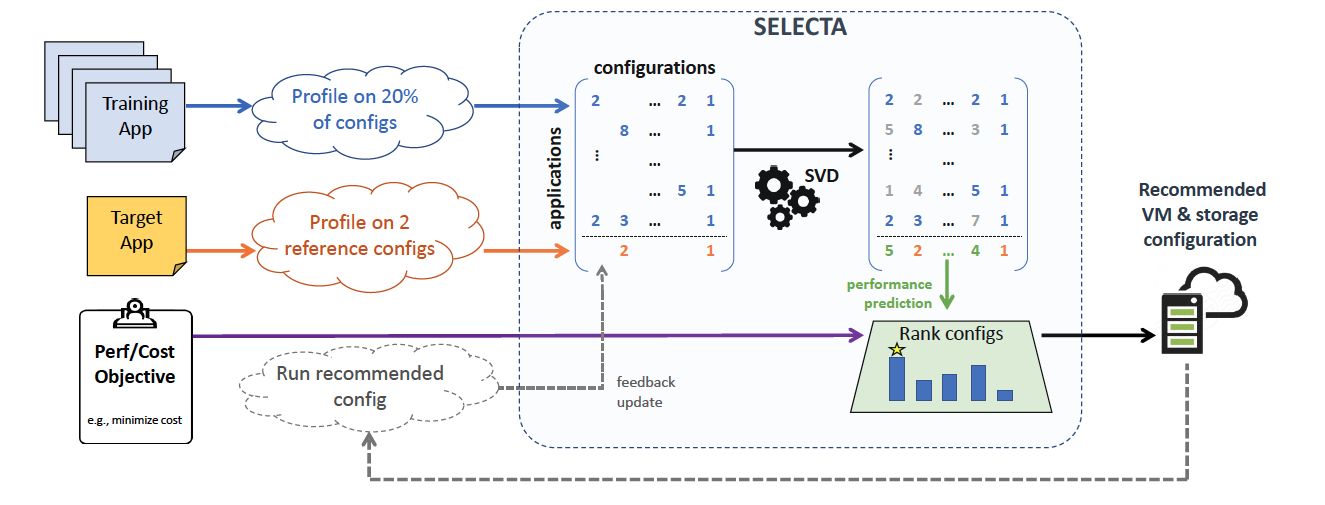
\includegraphics[width=\textwidth]{figures/selecta-arch.png}}
    \caption{Selecta系统架构。}
    \label{selecta_arch}
\end{figure}

随着深度学习模型的流行,也有研究者提出使用深度学习模型对应用性能进行建模,从而为应用选择最合适的云资源。F. Moradi\parencite{moradi2019performance}在2019年提出使用迁移学习算法实现通用的云应用性能预测。该方法先使用一个应用程序在所有的云配置上运行并收集性能数据,然后用深度神经网络对其建立性能模型,并将该模型计作基础模型。当需要为新的应用程序预测性能时,则抽出基础模型中的前若干层中的已训练参数放在新模型中,并使用新应用程序在少量配置上预运行得到结果对该模型进行微调,从而得到一个模型。该方法实际上是将已训练好的模型视作应用程序的特征抽取器,再使用其抽取的特征在新的数据上重新训练得到新模型。

基于上述工作,后续也有若干工作尝试在不同的应用场景下解决配置优化问题,但是总体上的方法皆大同小异。

\subsection{基于搜索的线上优化方法}
该类方法不同于数据驱动的线下建模方法,不需要在线下建立性能模型。其一般使用相关搜索算法(例如贝叶斯优化)在线上不断地搜索,并同时更新一个置信函数,当该函数值大于(或小于)某个阈值时,便停止搜索,用当前的到的数据中最优的一个作为结果。作为无需线下建模的纯线上方法,其固然具有其方便性。但是由于其掌握的信息过少,准确性一般要比基于线下建模的方式略低。

\begin{figure}[h]
    \centerline{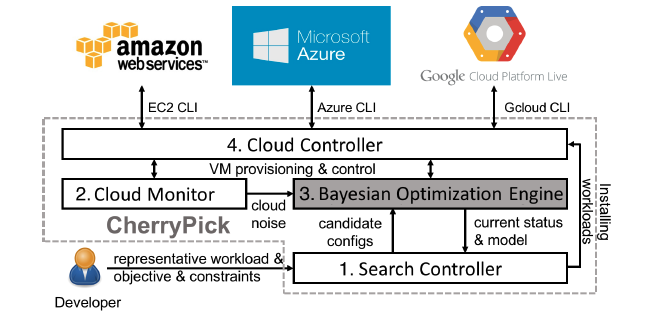
\includegraphics[width=\textwidth]{figures/cherrypick-arch.png}}
    \caption{CherryPick系统架构。}
    \label{cherrypick_arch}
\end{figure}

O. Alipourfard等人在2016年提出CherryPick\parencite{alipourfard2017cherrypick},使用典型的BO(Bayes Optimization,即贝叶斯优化)持续搜索不同的配置,直到其定义的置信函数超过某个阈值,则将当前搜索到的最优值作为最后的结果。图~\ref{cherrypick_arch}描述了CherryPick的系统架构,其支持在AWS,Azure和Google Cloud三家云厂商中对资源进行搜索,且支持用户自定义搜索的目标函数。

在CherryPick基础上,M. Casimiro等人在2020年提出了Lynceus\parencite{casimiro2019lynceus}。有别于CherryPick,Lynceus没有使用贪心的搜索方法,且不需要事先了解目标应用程序的任何信息。图~\ref{lynceus_arch}阐述了Lynceus与传统贝叶斯优化方法的区别所在。首先,Lynceus在考虑每一次搜索的reward的同时,还考虑了这一次搜索可能造成的cost。其实,传统的贝叶斯优化在一次尝试后即根据反馈推断下一次搜索的配置,Lynceus则是先预估一个可能的搜索路径,然后对路径的第一个节点进行尝试,最后得到最优结果。Lynceus更远的视野和更为精细的回报函数设计使得其相比于传统的贝叶斯优化拥有更高的准确率。

\begin{figure}[h]
    \centerline{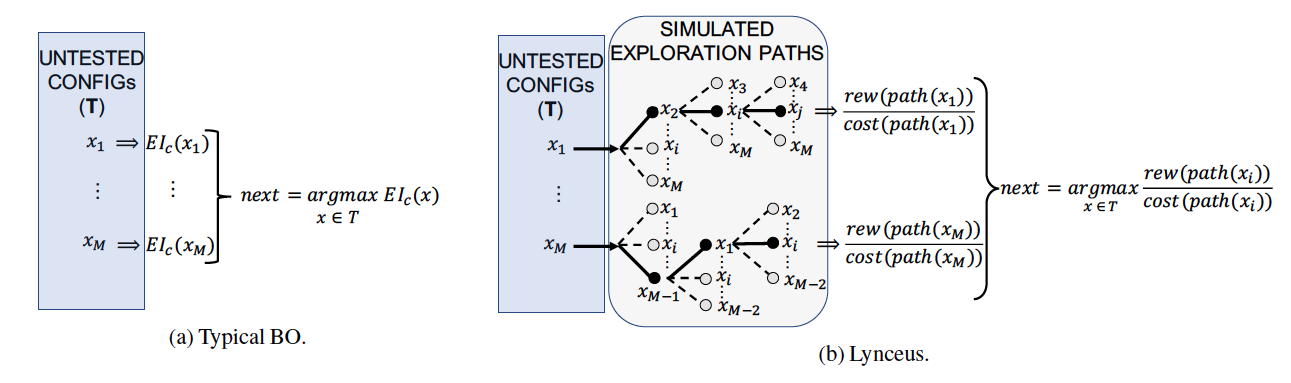
\includegraphics[width=\textwidth]{figures/lynceus-arch.png}}
    \caption{Lynceus与传统贝叶斯优化的区别。}
    \label{lynceus_arch}
\end{figure}

\section{基于机器学习算法的云资源调度优化技术}
资源调度是操作系统、分布式系统和云计算领域中的经典问题,其本质在于为系统中的每个任务分配合适的资源,从而使得系统达到某种状态,如资源利用率最高、闲置资源最少或者吞吐率最高等。近年来越来越多的学者开始尝试使用机器学习算法,特别是深度学习算法,对调度问题进行建模,试图更精确地解决调度问题。

C. Delimitrou等人在2014年提出了Quasar\parencite{delimitrou2014quasar},旨在保证作业性能的同时提升云上集群的资源利用率。Quasar和目前云计算厂商使用的资源预留策略(用户申请一定量的资源后即按照该量分配,即时相当一部分分配的资源处于空载状态)不同,而是要求用户提供一个动态的目标,使得集群调度器可以动态地适配其需要的资源。图~\ref{quasar_arch}展示了Quasar的系统架构。Quasar使用了协同过滤算法得到workload在满足QoS的前提下需要的资源数量和类型,以及会与那些workload产生干扰,再利用这一结果贪心地分配资源。通过实验,Quasar在200个EC2服务器的集群环境中提高了47\%的资源利用率。

\begin{figure}[h]
    \centerline{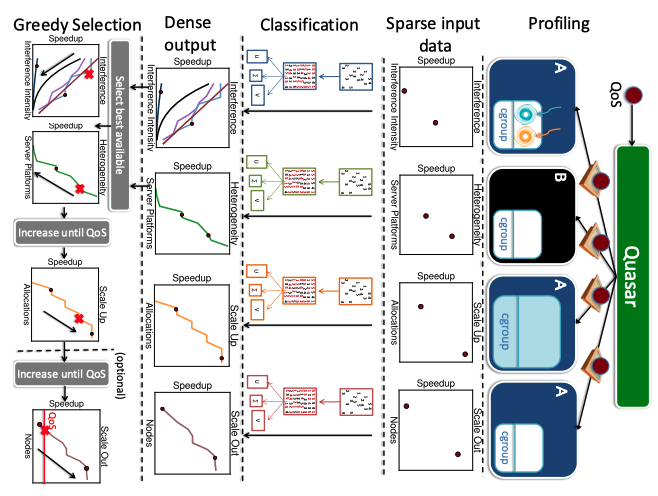
\includegraphics[width=\textwidth]{figures/quasar架构.png}}
    \caption{Quasar架构示意图。}
    \label{quasar_arch}
\end{figure}

随着深度学习的进一步发展,也有许多工作尝试将强化学习应用于调度问题。强化学习( Reinforcement Learning )是一种机器学习方法。这种方法通过与环境不断交互获得交互的反馈,从而获得经验,再从经验中不断学习,最终获得最优策略。其中经验(experience)是与环境交互得到的状态state)、动作action)和收益reward的采样序列。

H. Mao等人在2019年提出了Decima\parencite{mao2019learning},利用message passing等方法,将DAG作业的图结构建模到神经网络中,从而使得神经网络模型具有可扩展性,可适应任意作业队列长度的输入,而后通过policy gradient等强化学习方法训练调度器。结果显示Decima相比之前的启发式调度算法至少减少了21\%的平均作业完成时间。

除了使用强化学习算法,Decima中的另一个核心思想是使用图神经网络将DAG图中的作业节点编码成向量(亦称作embedding),再由这些向量生成Job级别的embedding和全局的embedding。这种思想借鉴于自然语言处理中的word2vec和图神经网络中的node2vec。如图~\ref{decima_embedding}所示,embedding生成的依据是DAG中各个节点之间的依赖关系。这样做的好处是将图中节点的依赖关系转化为高维空间中向量之间的代数关系,使得模型能够更容易的学习到规律。

\begin{figure}[h]
    \centerline{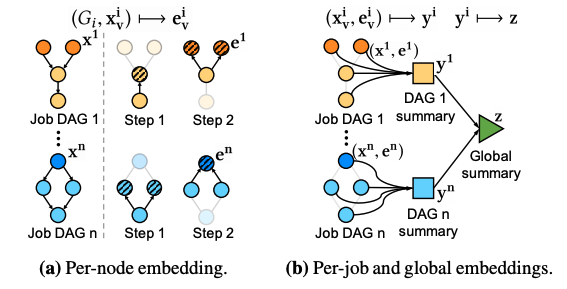
\includegraphics[width=\textwidth]{figures/decima-embedding.png}}
    \caption{Decima中的embedding生成示意图。}
    \label{decima_embedding}
\end{figure}

F. Li等人在2019年提出了DeepJS\parencite{li2019deepjs},将问题模型化为选择机器-作业对的问题,每次调度前构造可行的机器作业对列表,由神经网络输出每个对的得分,优先调度得分高的机器作业对。A. Mirhoseini等\parencite{mirhoseini2017device}使用强化学习算法训练了Tensorflow计算操作的放置策略(放置于哪个计算设备,如CPU),它使用了一种循环神经网络去编码状态,而不是采用具有可扩展性的图神经网络。

\begin{figure}[h]
    \centerline{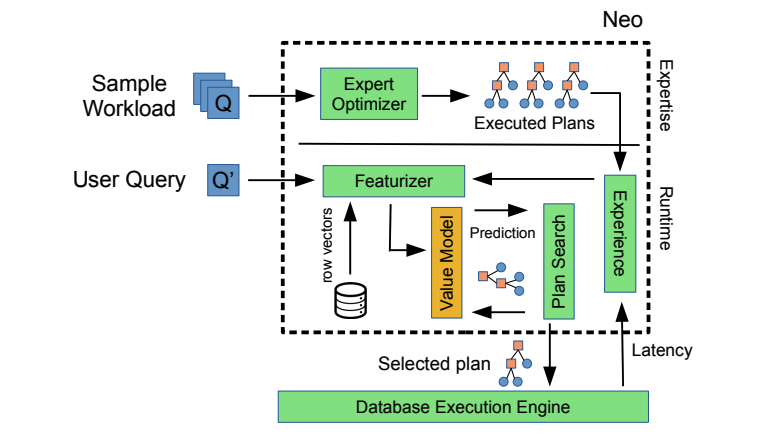
\includegraphics[width=\textwidth]{figures/neo-arch.png}}
    \caption{Neo系统架构示意图。}
    \label{neo_arch}
\end{figure}

受到Decima的启发,有一些学者开始考虑将深度学习算法和图神经网络应用到云数据库中的查询优化中,因为数据库中的一次查询所对应的语法树天生就是一个DAG图,图的节点对应数据库中的operator。R. Marcus等人在2019年提出Neo\parencite{marcus2019neo},一种基于深度学习的数据库查询优化器。图~\ref{neo_arch}阐述了Neo的系统架构。与~\ref{sec_profling}中所述的基于线下模型训练的性能预测方法类似,Neo需要先使用sample workload,通过一个已有的最优优化器(可能是基于专家的经验,也可能基于历史信息),构建一个查询优化的信息库(即图中的Experience)。当用户发起查询时,Neo中的特征提取器会结合经验和用户的查询语句对其进行特征提取。此处的特征提取Neo使用了树形的卷积网络对语句中的operator进行编码,然后做出决策,交由数据库引擎执行。T. Kraska在2019年也提出了一个基于深度学习的数据库系统SageDB\parencite{47669}。和Neo相比,SageDB更进一步,其在数据库查询执行、数据预取等阶段都利用机器学习模型做了相关优化

\section{小结}

本节从用户和云厂商运营者两个角度,研究了云计算中的两个经典问题,即云资源配置优化与云资源调度。基于机器学习的云资源配置优化技术正在经历从支持特定领域应用向支持通用应用的发展历程。未来,关于如何用较小的代价获取通用性较强的资源配置优化模型,将会是研究的重点。基于机器学习的资源调度算法一般都是将资源调度问题抽象为典型的机器学习领域的问题,例如通过协同过滤算法建立不同实体之间的关系,利用图神经网络对DAG图的节点进行编码,利用强化学习不断调整系统的状态等等。事实上,利用机器学习算法解决调度问题目前亦处于探索阶段。大型分布式系统中,往往要求调度器能够快速做出决策,而基于机器学习尤其是深度学习的调度模型,往往具有较高的延时,可能会给系统带来过重的额外开销。未来,除了使调度算法做出更优的决策之外,尝试降低基于ML的调度算法的额外开销,也会是一个可能的研究方向。
	\chapter{重要文献与研究团队总结}

\section{重要文献总结}

\section{重要研究团队总结}
	\chapter{下一步的研究设想}

\section{研究动机}

作者现阶段的研究设想均与机器学习模型部署相关。一个是在新的云计算服务模式下的进行模型部署,另一个是在安全计算环境SGX中进行模型部署。二者所要达到的目的也类似,即在保证服务质量的前提下,尽量提升集群的资源利用率。

\subsection{基于FaaS的模型部署系统现状}
serverless是一种非常适合部署ML模型的计算模式,其具有细粒度计费、横向拓展能力强的特点。但是现有的serverless框架用来做ML模型部署时,仍然存在一定的问题;
\begin{itemize}
    \item 当前公有云的serverless服务仅使用CPU,单个servereless实例没有并发能力,能够满足的吞吐量有限。而横向拓展又会因为冷启动造成延迟增加,可能会违背任务的SLO。
    \item serverless一般是基于容器技术实现的(例如Docker等)。而容器使用GPU一般是独占的方式(nvidia-docker),这样会造成显存浪费。通过实验可以证明,在满足一定SLO的前提下,batching的上限距离显存大小仍有一定的差距。
\end{itemize}

如果能解决上述问题,将GPU共享机制和基于SLO的显存调度机制引入serverless系统中,可能可以在保证服务质量的前提下大幅提升系统的资源利用率。

\subsection{基于SGX的模型部署系统现状}
基于SGX的模型部署系统在真实场景中有着广泛的需求,尽管学术界已经在这方面做了一些探索,但是仍有如下问题需要解决:
\begin{itemize}
    \item 由于SGX目前所支持的EPC大小有限,共同部署在同一个EPC内的模型之间可能会存在干扰。
    \item 由于SGX本身的封闭性,对于部署SGX的Enclave内部的应用很难直接对其EPC利用率进行直接监测,从而获得该应用的行为信息(例如内存利用率的变化模式)。
\end{itemize}

如果能解决上述问题,通过一个工具预测应用在SGX环境下的干扰情况,再基于此实现调度算法,则可以在保证SGX环境下模型部署服务质量的前提下,提升SGX集群的资源利用率。

%\subsection{基于线下数据建模的云资源配置推荐现状}

\section{研究设想}

\subsection{SLO可感知的Serverless机器学习模型部署系统}
为了让用户在云上在满足SLO的条件下更cost-efficient的使用serverless部署ML模型,本文拟提出一种SLO-aware的基于GPU显存sharing的serverless框架,解决如下问题:
\begin{itemize}
    \item 实现一种基于API截取的GPU显存共享中间件,使得多个容器可以共享同一块GPU,且相互之间隔离。
    \item 使用GPU的serverless实例时,根据服务的SLO计算其能容许的batching的请求上限,划分一块显存给其使用。
    \item 基于上述机制,实现一种SLO可感知的服务调度算法,将若干服务按照其SLO对应的显存上限进行调度,使多个服务可以在一个GPU设备上共存,提高系统资源利用率。
\end{itemize}

\subsection{SGX环境下机器学习模型部署干扰及调度策略研究}
为了能在SGX更高效地部署机器学习模型,本文拟提出一种SGX环境下机器学习模型部署干扰的建模方法,以及基于此的模型部署服务调度算法:
\begin{itemize}
    \item 在非SGX的环境中对应用(此处的应用对应机器学习模型部署服务)运行时系统信息(例如CPU利用率的变化曲线,与内存相关的指标如换页频率、内存利用率的变化曲线)进行收集,分析应用的行为模式。
    \item 在SGX的环境中部署多个应用,研究其相互干扰的情况。
    \item 将上述两个信息利用模型建立关系,得到一个预测应用之间干扰程度的工具。
    \item 利用上述工具,实现一种SGX环境下的应用调度算法,通过对应用在非SGX环境中采集少许运行时数据,预测其可能与系统中现存的服务之间的干扰关系,将其调度到最合适的节点上。
\end{itemize}

%\subsection{结合频域信息对数据处理类任务进行更精确的建模}

	% 正文中的附录部分。
	\appendix
	% 排版参考文献列表。bibintoc 选项使“参考文献”出现在目录中;
	% 如果同时要使参考文献列表参与章节编号,可将“bibintoc”改为“bibnumbered”。
	\printbibliography[heading = bibintoc]
	% 各附录。
	%\include{chap/encl1}

	% 以下为正文之后的部分,默认不进行章节编号。
	%\backmatter
	% 致谢。
	%\ifblind\else\include{chap/ack}\fi
	% 原创性声明和使用授权说明。
	%\include{chap/origin}
\end{document}

% vim:ts=4:sw=4
